\chapter{Geometry creation}\label{chap:GeometryCreation}
The creation of geometry objects within the computational domain is
a crucial part of the simulation process.  This chapter discusses the
options avialble for creating geometry in \Vaango.

\section{Basic geometry objects} \label{Sec:GeometryObjects}

Each geometry object has the following properties, label (string
name), type (box, cylinder, sphere, etc), resolution (vector
quantity), and any unique geometry parameters such as origin, corners,
triangulated data file, etc.  The operators which include, the union,
the difference, and intersection tags contain either lists of
additional operators or the primitives pieces.

As an example of a non-trivial geometry object is shown below:

\begin{lstlisting}[language=XML]
<geom_object>
     <intersection>
       <box label = "Domain">
          <min>[0.0,0.0,0.0]</min>
          <max>[0.1,0.1,0.1]</max>
       </box>
       <union>
         <sphere label = "First node">
            <origin>[0.022,0.028,0.1  ]</origin>
            <radius>0.01</radius>
         </sphere>
         <sphere label = "2nd node">
            <origin>[0.030,0.075,0.1  ]</origin>
            <radius>0.01</radius>
         </sphere>
       </union>
     </intersection>
     <res>[2,2,2]</res>
     <velocity>[0.,0.,0.]</velocity>
     <temperature>0 </temperature>
</geom_object>
\end{lstlisting}

The following geometry objects are given with their required tags:

\subsection{Box}
\begin{minipage}{0.6\textwidth}
  \Textsfc{box} requires the tags \Textsfc{min} and \Textsfc{max} which are
  vector quantities specified in the \Textsfc{[a, b, c]} format.
  \begin{lstlisting}[language=XML]
    <box label="box_1">
      <min>[0.0, 0.0, 0.0]</min>
      <max>[1.0, 2.0, 3.0]</max>
    </box>
  \end{lstlisting}
\end{minipage}
\begin{minipage}{0.4\textwidth}
  \centering
  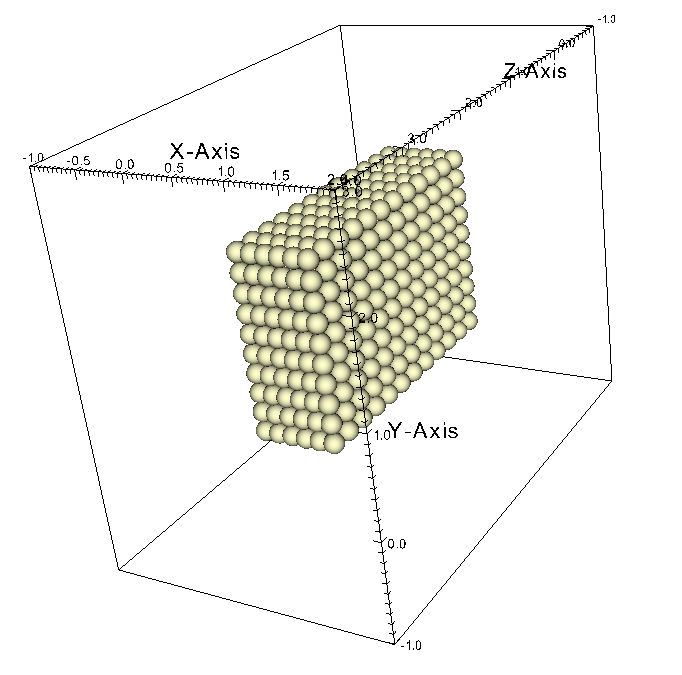
\includegraphics[width=0.9\columnwidth]{FIGS/geometry/geom_box.png}
  \captionof{figure}{A \Textsfc{box} geometry piece.}
\end{minipage}

\subsection{Parallelepiped}
\begin{minipage}{0.6\textwidth}
  \Textsfc{parallelepiped} requires the locations of four points
  that define the bounds of the parallelepiped.  The point \Textsfc{p1}
  is a corner while the the vectors \Textsfc{p2 - p1}, \Textsfc{p3 - p1},
  and \Textsfc{p4 - p1} represent the vectors along the three edges
  of the parallelepiped starting from \Textsfc{p1}.
  \begin{lstlisting}[language=XML]
    <parallelepiped label="box_1">
      <p1>[ 0.0, 0.0, 0.0]</p1>
      <p2>[ 1.0, 0.0, 0.0]</p2>
      <p3>[ 1.0, 2.0, 0.5]</p3>
      <p4>[-1.0, 1.0, 2.0]</p4>
    </parallelepiped>
  \end{lstlisting}
  \centering
  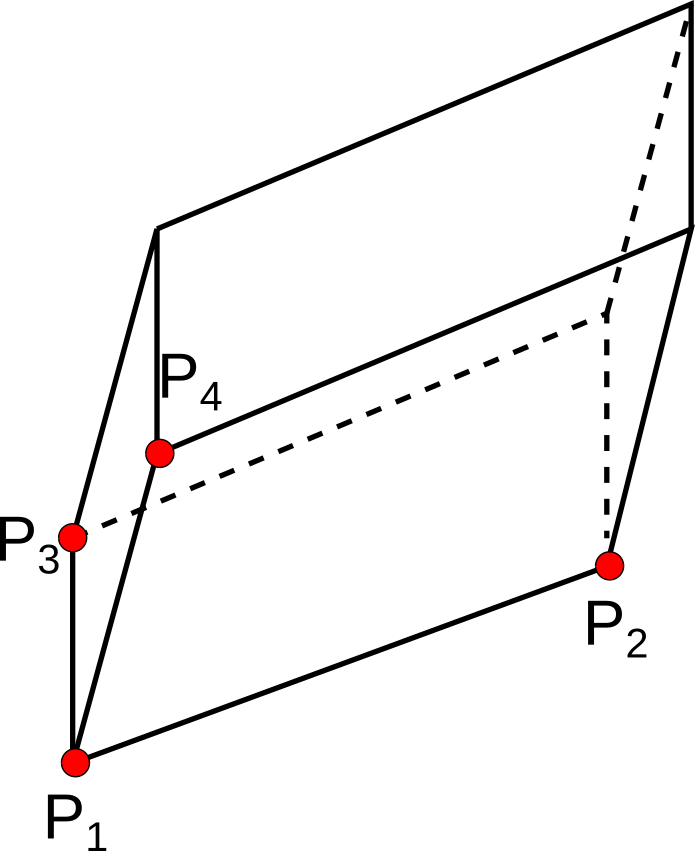
\includegraphics[width=0.3\columnwidth]{FIGS/geometry/naa_box_def.png}
\end{minipage}
\begin{minipage}{0.4\textwidth}
  \centering
  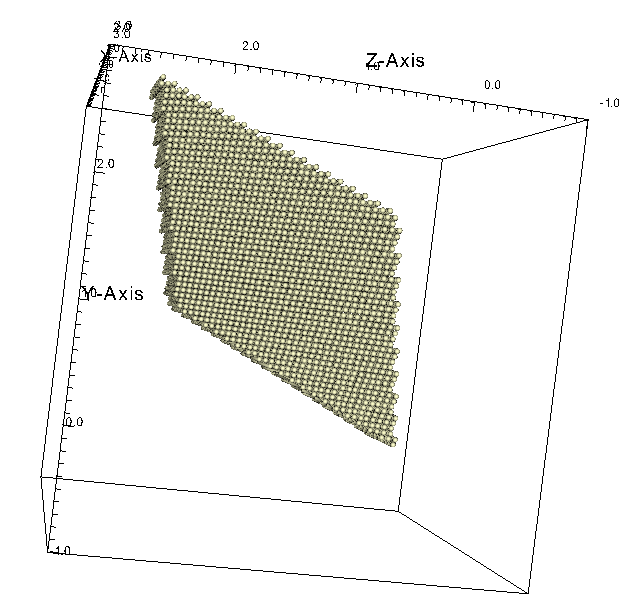
\includegraphics[width=0.9\columnwidth]{FIGS/geometry/geom_naa_box.png}
  \captionof{figure}{A \Textsfc{parallelepiped} geometry piece.}
\end{minipage}

\subsection{Sphere}
\begin{minipage}{0.6\textwidth}
  \Textsfc{sphere} has an \Textsfc{origin} tag specified as a vector and the
  \Textsfc{radius} tag specified as a float.
  \begin{lstlisting}[language=XML]
    <sphere label="ball_1">
      <origin>[ 0.0, 0.0, 0.0]</origin>
      <radius> 0.75 </radius>
    </sphere>
  \end{lstlisting}
\end{minipage}
\begin{minipage}{0.4\textwidth}
  \centering
  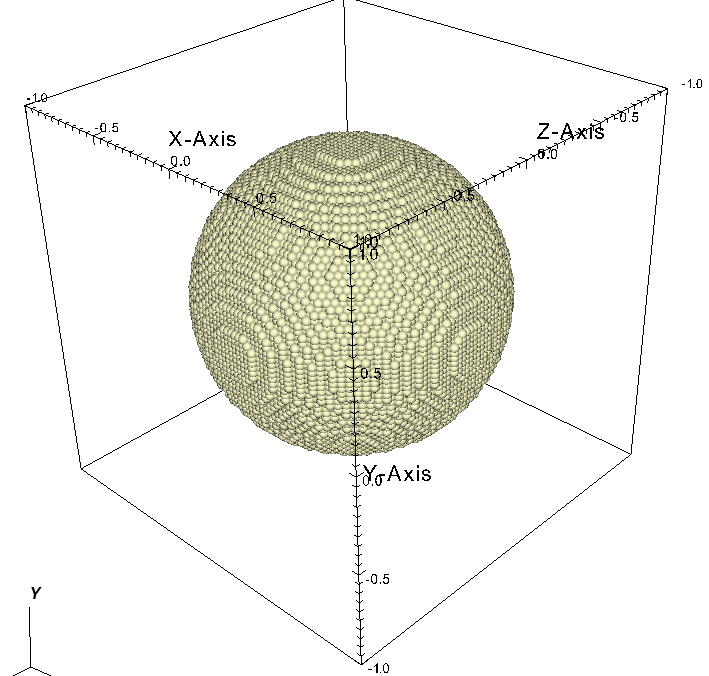
\includegraphics[width=0.9\columnwidth]{FIGS/geometry/geom_sphere.png}
  \captionof{figure}{A \Textsfc{sphere} geometry piece.}
\end{minipage}

\subsection{Cylinder}
\begin{minipage}{0.6\textwidth}
  \Textsfc{cylinder} has a tag for the \Textsfc{top} and \Textsfc{bottom} origins
  (vector) plus a tag for the \Textsfc{radius} (float).
  \begin{lstlisting}[language=XML]
    <cylinder label="cyl_1">
      <bottom>[ -0.5, -0.5, -0.5]</bottom>
      <top>[ 1.5, 1.5, 1.5]</top>
      <radius> 0.5 </radius>
    </cylinder>
  \end{lstlisting}
\end{minipage}
\begin{minipage}{0.4\textwidth}
  \centering
  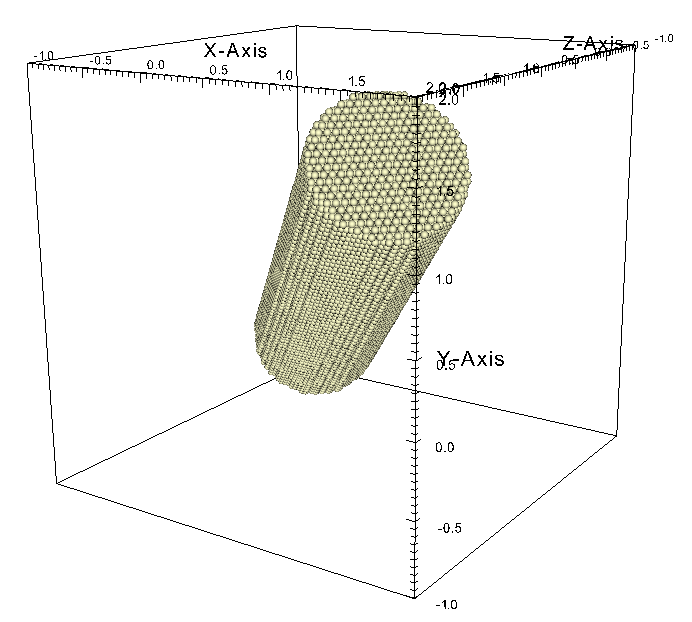
\includegraphics[width=0.9\columnwidth]{FIGS/geometry/geom_cyl.png}
  \captionof{figure}{A \Textsfc{cylinder} geometry piece.}
\end{minipage}

\subsection{Cone}
\begin{minipage}{0.6\textwidth}
  \Textsfc{cone} has a tag for the \Textsfc{top} and \Textsfc{bottom} origins (vector)
  as well as tags for the top and bottom \Textsfc{radius} (float) to create a
  right circular cone/frustum.
  \begin{lstlisting}[language=XML]
    <cone label="cone_1">
      <bottom>[ -0.5, -0.5, -0.5]</bottom>
      <top>[ 1.5, 1.5, 1.5]</top>
      <bottom_radius> 0.7 </bottom_radius>
      <top_radius> 0.1 </top_radius>
    </cone>
  \end{lstlisting}
\end{minipage}
\begin{minipage}{0.4\textwidth}
  \centering
  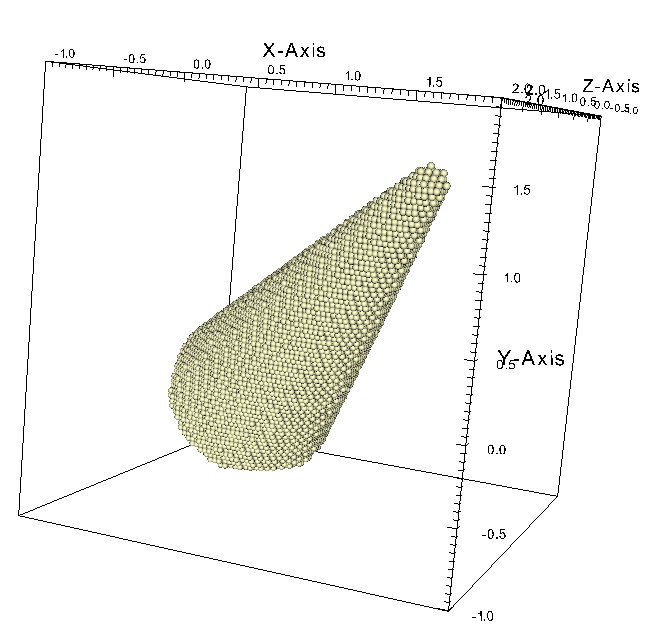
\includegraphics[width=0.9\columnwidth]{FIGS/geometry/geom_cone.png}
  \captionof{figure}{A \Textsfc{cone} geometry piece.}
\end{minipage}

\subsection{Ellipsoid}
\begin{minipage}{0.6\textwidth}
  \Textsfc{ellipsoid} has an \Textsfc{origin} tag specified as a vector.  
  An ellipsoid is defined by two orthogonal axis vectors \Textsfc{v1} and
  \Textsfc{v2} and three semi-axis lengths \Textsfc{r1}, \Textsfc{r2}, \Textsfc{r3}.
  The axis vectors must be orthogonal to within 1e-12 after dot product or 
  the simulation will throw an exception.  
  \begin{lstlisting}[language=XML]
    <ellipsoid label="ellipsoid_1">
      <origin>[ 0.0, 0.0, 0.0]</origin>
      <v1> [0.353553, 0.353553, 0.4] </v1>
      <v2> [0.087038295569, -0.783349583783, 0.615457362205] </v2>
      <r1> 0.6403119924052649 </r1>
      <r2> 1.0 </r2>
      <r3> 2.0 </r3>
    </ellipsoid>
  \end{lstlisting}
\end{minipage}
\begin{minipage}{0.4\textwidth}
  \centering
  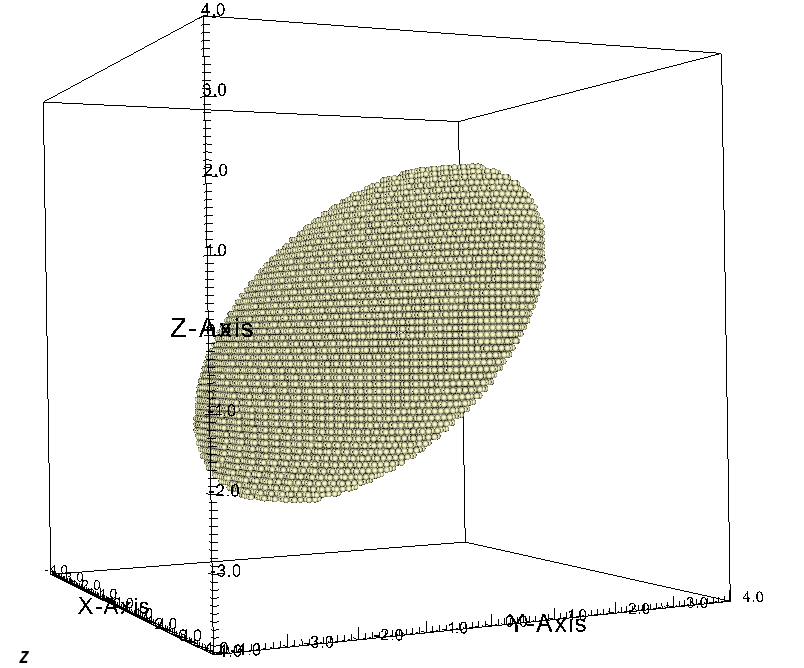
\includegraphics[width=0.9\columnwidth]{FIGS/geometry/geom_ellipsoid.png}
  \captionof{figure}{An \Textsfc{ellipsoid} geometry piece.}
\end{minipage}

\subsection{Torus}
\begin{minipage}{0.6\textwidth}
  \Textsfc{torus} has a \Textsfc{center}, an \Textsfc{axis} vector,
  and \Textsfc{major} and \Textsfc{minor} radii.   The major radius must
  be greater than the minor radius.  The axis vector is converted
  internally into a unit vector and cannot have zero length.
  \begin{lstlisting}[language=XML]
    <torus label="torus object">
      <center> [0.1, 0.1, 0.1] </center>
      <axis_vector>[ 1.5, 1.5, 1.5] </axis_vector>
      <major_radius> 1.0 </major_radius>
      <minor_radius> 0.5 </minor_radius>
    </torus>
  \end{lstlisting}
\end{minipage}
\begin{minipage}{0.4\textwidth}
  \centering
  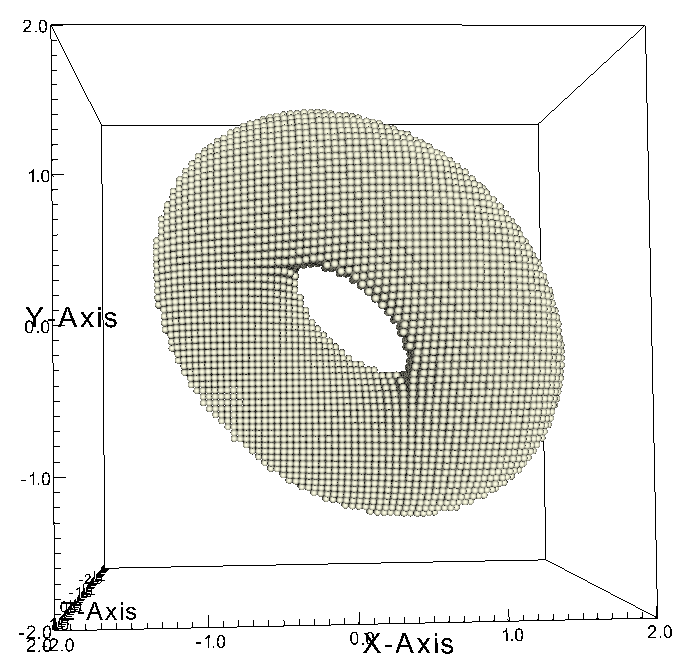
\includegraphics[width=0.6\columnwidth]{FIGS/geometry/geom_torus.png}
  \captionof{figure}{A \Textsfc{torus} geometry piece.}
\end{minipage}

\subsection{Triangulated surface}
\begin{minipage}{0.7\textwidth}
  \Textsfc{tri} is a tag for describing a triangulated surface.
  The \Textsfc{file\_name\_prefix} tag specifies the file name to use for reading in the
  triangulated surface description and the points file.  
  \begin{lstlisting}[language=XML]
    <tri label = "goblet">
      <file_name_prefix> tri_goblet </file_name_prefix>
    </tri>
  \end{lstlisting}
  The default behavior is to expect a triangulated surface file (\Textbfc{file\_name.tri}) 
  that contains a list of integers
  describing the connectivity of points specified in \Textbfc{file\_name.pts}.
  Here is an excerpt from the \Textbfc{tri\_goblet.tri} file:
  \begin{lstlisting}[backgroundcolor=\color{background}]
  0 49 6
  0 6 18
  18 6 8
  18 8 22
  ....
  \end{lstlisting}
  The \Textbfc{tri\_goblet.pts} file contains data of the form:
  \begin{lstlisting}[backgroundcolor=\color{background}]
  -2.6575 -0.366357 2.656
  -2.69162 -0.57185 2.656
  -2.61027 -0.577179 2.53656
  -2.69395 -0.641317 2.656
  -2.5085 -0.406282 2.39336
  ....
  \end{lstlisting}
  The \Textsfc{tri} tag can also be used to read triangulated surfaces in \Textbfc{OBJ}, 
  \Textbfc{PLY}, and \Textbfc{STL} formats.  The \Textsfc{file\_type} tag specifies the 
  type of file to be read.  For a \Textbfc{PLY} file, the file has to have the \Textsfc{.stl}
  extension and we can use the following:
  \begin{lstlisting}[language=XML]
    <tri label = "horse">
      <file_name_prefix> horse </file_name_prefix>
      <file_type> ply </file_type>
    </tri>
  \end{lstlisting}
  For an \Textbfc{OBJ} file, with extension \Textsfc{.obj}, we need
  \begin{lstlisting}[language=XML]
    <tri label = "teddy bear">
      <file_name_prefix> teddy </file_name_prefix>
      <file_type> obj </file_type>
    </tri>
  \end{lstlisting}
  For a \Textbfc{STL} file, with extension \Textsfc{.stl}, the UPS file requires
  \begin{lstlisting}[language=XML]
    <tri label = "panther">
      <file_name_prefix> panther </file_name_prefix>
      <file_type> stl </file_type>
    </tri>
  \end{lstlisting}
\end{minipage}
\begin{minipage}{0.3\textwidth}
  \centering
  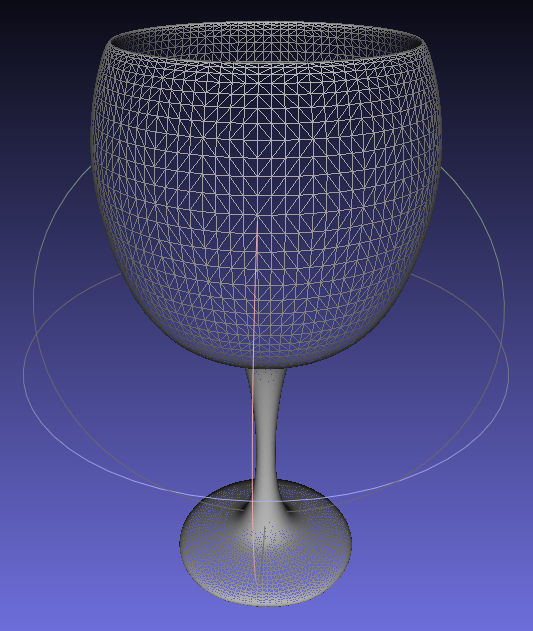
\includegraphics[width=0.6\columnwidth]{FIGS/geometry/geom_tri_mesh.png}
  \captionof{figure}{The triangle mesh.}
  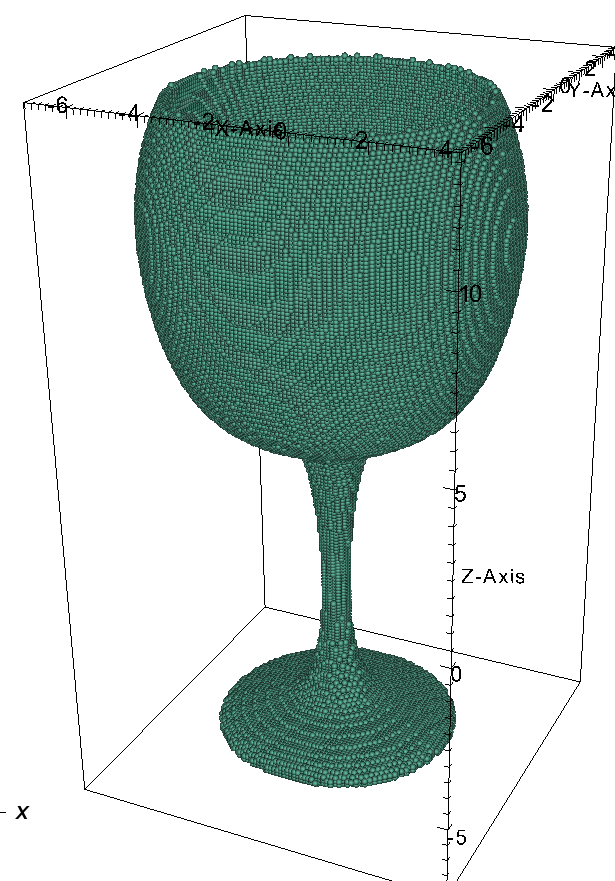
\includegraphics[width=0.6\columnwidth]{FIGS/geometry/geom_tri.png}
  \captionof{figure}{A \Textsfc{tri} geometry piece.}
  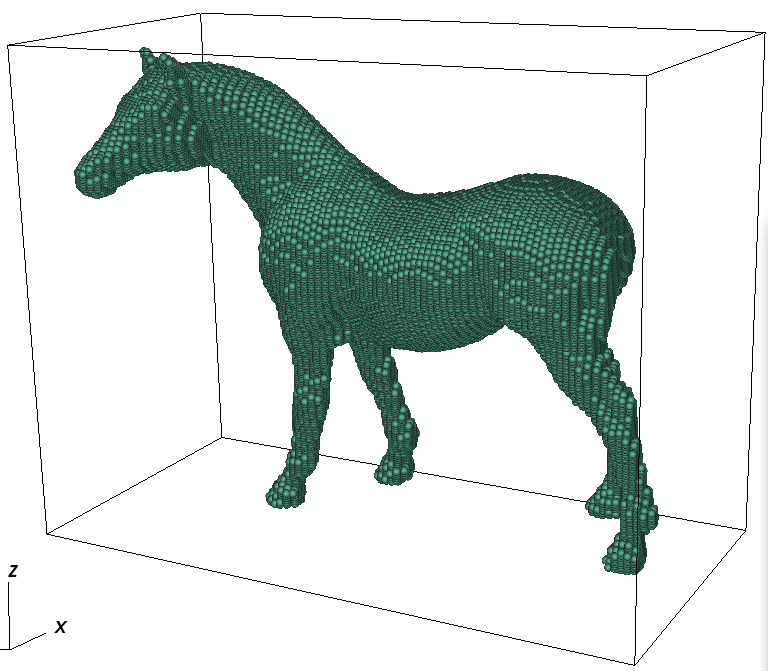
\includegraphics[width=0.7\columnwidth]{FIGS/geometry/geom_tri_ply.png}
  \captionof{figure}{Particles created from a PLY mesh.}
\end{minipage}

\begin{minipage}{0.6\textwidth}
  \begin{NoteBox}
  If you are unsure of the size of the domain that will fit your geometry,
  examine the output to get information on the bounding box of the object that
  has been read in.
  \end{NoteBox}
  \Textsfc{tri} geometry pieces can \Textsfc{scaled}, \Textsfc{reflected}, and 
  \Textsfc{translated}.  The \Textsfc{order} of the co-ordinates can also be
  rearranged to suit a given simulation.

  To scale an object we use the \Textsfc{scaling\_factor} tag:
  \begin{lstlisting}[language=XML]
    <tri label = "panther">
      <file_name_prefix> panther </file_name_prefix>
      <file_type> stl </file_type>
      <scaling_factor> 0.5 </scaling_factor>
    </tri>
  \end{lstlisting}

  To translate an object we use the \Textsfc{translation\_vector} tag:
  \begin{lstlisting}[language=XML]
    <tri label = "panther">
      <file_name_prefix> panther </file_name_prefix>
      <file_type> stl </file_type>
      <scaling_factor> 0.5 </scaling_factor>
      <translation_vector> [0.0, -15.0, 0.0] </translation_vector>
    </tri>
  \end{lstlisting}

  To reflect an object about an axis we use the \Textsfc{reflection\_vector} tag.
  Reflections are currently allowed only with reflect to the global coordinates
  and require a value of -1 to reflect and 1 to retain the current orientation.
  \begin{lstlisting}[language=XML]
    <tri label = "panther">
      <file_name_prefix> panther </file_name_prefix>
      <file_type> stl </file_type>
      <scaling_factor> 0.5 </scaling_factor>
      <reflection_vector> [1.0, 1.0, -1.0] </reflection_vector>
    </tri>
  \end{lstlisting}

  The order of the axes can also be change during the geometry set-up phase
  to align the object along a particular orientation.  The \Textsfc{axis\_sequence}
  tag is used for that purpose.  Allowed values are $[1,2,3]$, $[2,3,1]$, $[3,1,2]$,
  $[1,3,2]$ , $[3,2,1]$, and $[2,1,3]$.
  \begin{lstlisting}[language=XML]
    <tri label = "panther">
      <file_name_prefix> panther </file_name_prefix>
      <file_type> stl </file_type>
      <scaling_factor> 0.5 </scaling_factor>
      <axis_sequence> [2,1,3] </axis_sequence>
    </tri>
  \end{lstlisting}

  \begin{WarningBox}
  The order in which the scaling, translation, and reflection operations are carried
  out matters.  Translation followed by scaling will lead to different results than 
  scaling followed by translation.  The same holds for rfelection.  Internally, objects
  are scaled first, reflected, and then translated.
  \end{WarningBox}
\end{minipage}
\hspace{12pt}
\begin{minipage}{0.35\textwidth}
  \centering
  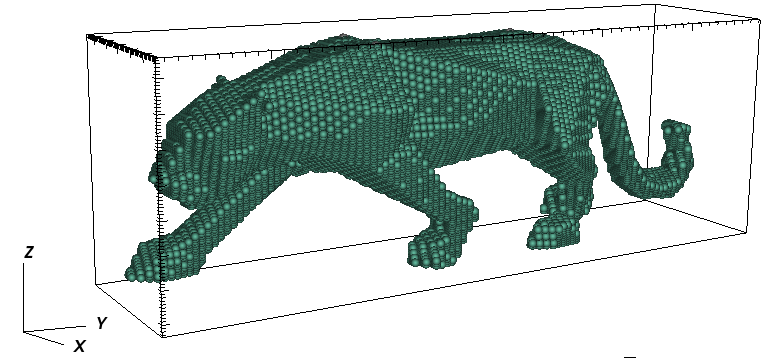
\includegraphics[width=\columnwidth]{FIGS/geometry/geom_tri_stl.png}
  \captionof{figure}{Particles created from a STL mesh.}
  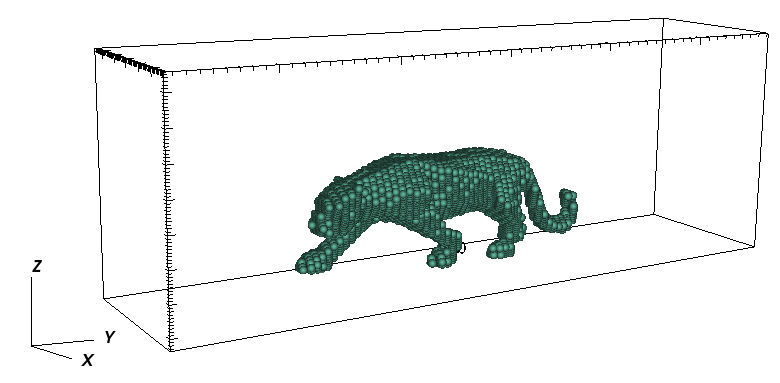
\includegraphics[width=\columnwidth]{FIGS/geometry/geom_tri_stl_scale.png}
  \captionof{figure}{Scaled geometry.}
  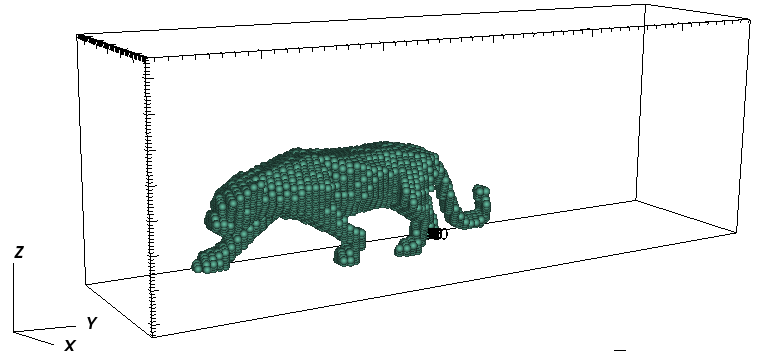
\includegraphics[width=\columnwidth]{FIGS/geometry/geom_tri_stl_translate.png}
  \captionof{figure}{Scaled and translated geometry.}
  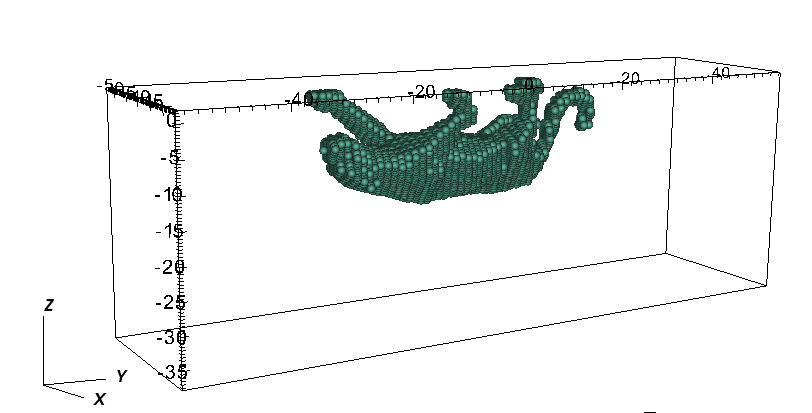
\includegraphics[width=\columnwidth]{FIGS/geometry/geom_tri_stl_reflect.png}
  \captionof{figure}{Reflected geometry in $z$-direction.}
  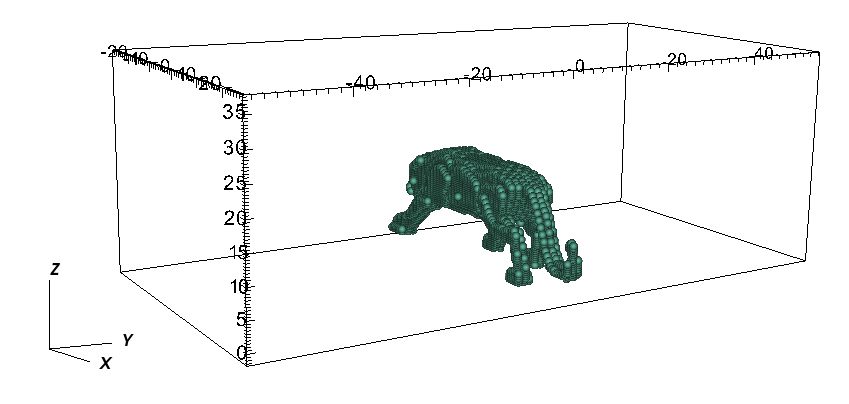
\includegraphics[width=\columnwidth]{FIGS/geometry/geom_tri_stl_sequence.png}
  \captionof{figure}{Change of coordinate sequence.}
\end{minipage}

\subsection{Boolean operations}
The boolean operators on the geometry pieces include \Textsfc{difference,
intersection,} and \Textsfc{union}.
Multiple operators can be used to form very complex geometry pieces.

\begin{minipage}{0.6\textwidth}
  The \Textsfc{difference} takes two geometry pieces and subtracts
  the second geometry piece from the first geometry piece.  
  \begin{lstlisting}[language=XML]
    <difference>
      <box label="box_1">
        <min>[-0.75, -0.75, -0.75]</min>
        <max>[ 0.75,  0.75,  0.75]</max>
      </box>
      <sphere label="ball_1">
        <origin>[ 0.0, 0.0, 0.0]</origin>
        <radius> 1.00 </radius>
      </sphere>
    </difference>
  \end{lstlisting}
  \begin{lstlisting}[language=XML]
    <difference>
      <sphere label="ball_1">
        <origin>[ 0.0, 0.0, 0.0]</origin>
        <radius> 1.00 </radius>
      </sphere>
      <box label="box_1">
        <min>[-0.75, -0.75, -0.75]</min>
        <max>[ 0.75,  0.75,  0.75]</max>
      </box>
    </difference>
  \end{lstlisting}
\end{minipage}
\begin{minipage}{0.4\textwidth}
  \centering
  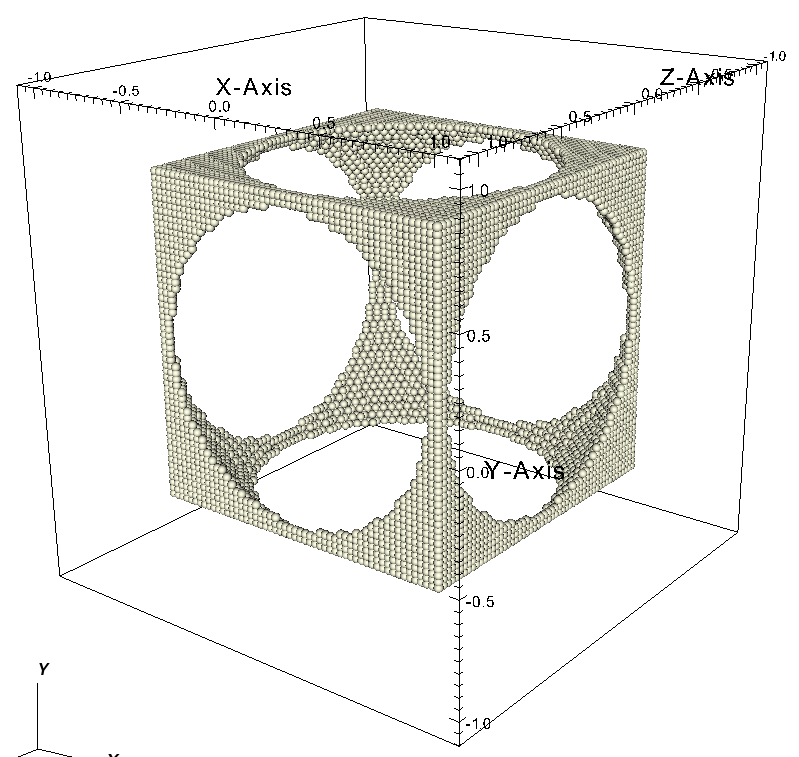
\includegraphics[width=0.7\columnwidth]{FIGS/geometry/geom_diff_12.png}
  \captionof{figure}{The \Textsfc{difference} of a sphere from a cube.}
  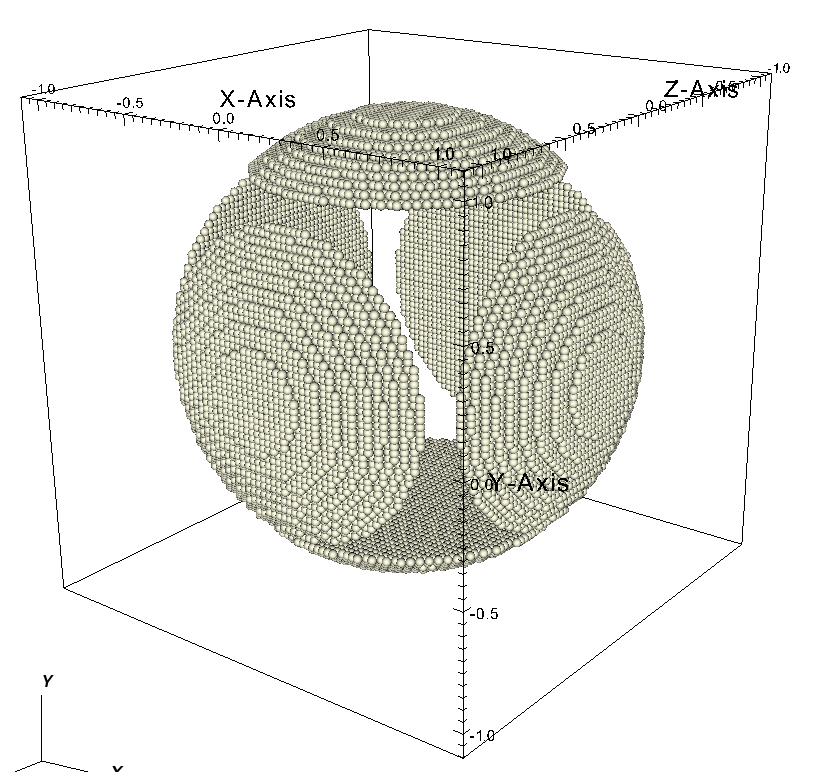
\includegraphics[width=0.7\columnwidth]{FIGS/geometry/geom_diff_21.png}
  \captionof{figure}{The \Textsfc{difference} of a cube from a sphere.}
\end{minipage}

\begin{minipage}{0.6\textwidth}
  The \Textsfc{intersection} operator requires at least two geometry
  pieces in forming an intersection geometry piece.  
  \begin{lstlisting}[language=XML]
    <intersection>
      <box label="box_1">
        <min>[-0.75, -0.75, -0.75]</min>
        <max>[ 0.75,  0.75,  0.75]</max>
      </box>
      <sphere label="ball_1">
        <origin>[ 0.0, 0.0, 0.0]</origin>
        <radius> 1.00 </radius>
      </sphere>
    </intersection>
  \end{lstlisting}
\end{minipage}
\begin{minipage}{0.4\textwidth}
  \centering
  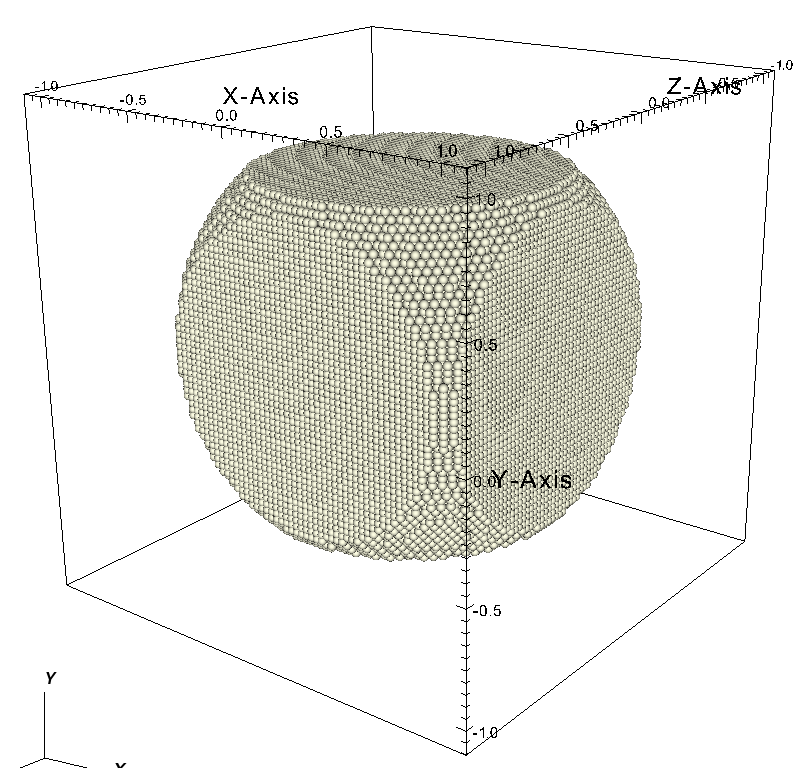
\includegraphics[width=0.7\columnwidth]{FIGS/geometry/geom_intersect.png}
  \captionof{figure}{An \Textsfc{intersection} of a sphere and a cube.}
\end{minipage}

\begin{minipage}{0.6\textwidth}
  The \Textsfc{ union} operator aggregates a collection of geometry pieces.
  \begin{lstlisting}[language=XML]
    <union>
      <box label="box_1">
        <min>[-0.75, -0.75, -0.75]</min>
        <max>[ 0.75,  0.75,  0.75]</max>
      </box>
      <sphere label="ball_1">
        <origin>[ 0.0, 0.0, 0.0]</origin>
        <radius> 1.00 </radius>
      </sphere>
    </union>
  \end{lstlisting}
\end{minipage}
\begin{minipage}{0.4\textwidth}
  \centering
  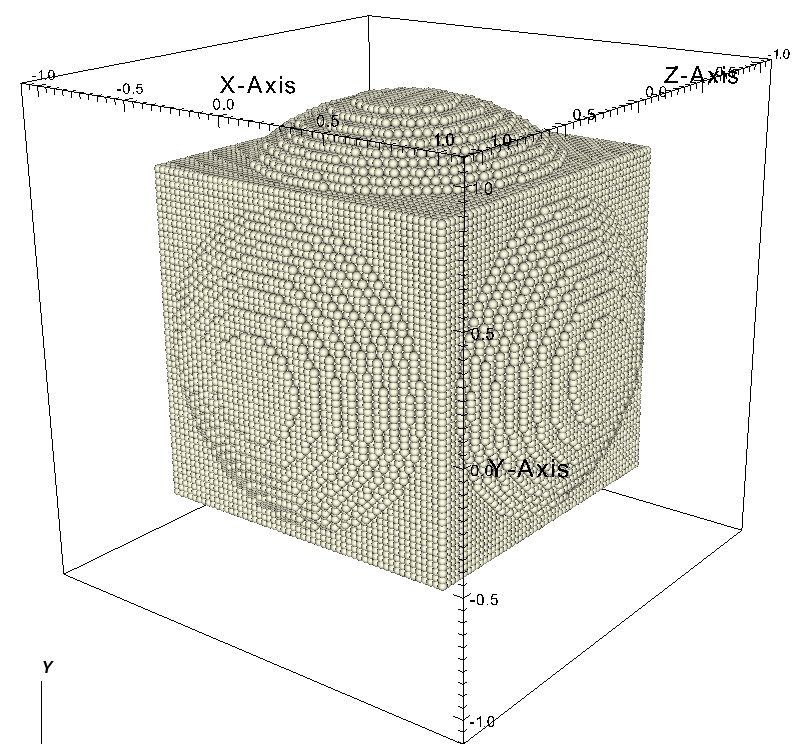
\includegraphics[width=0.7\columnwidth]{FIGS/geometry/geom_union.png}
  \captionof{figure}{A \Textsfc{union} of a sphere and a cube.}
\end{minipage}

\section{Special geometry objects} \label{Sec:SpecialGeometryObjects}
A few special geometry objects exist that do not force the material points
to be distributed according to the geometry of the background grid.
These are discussed below.

\subsection{Smooth Cylinder}
\begin{minipage}{0.6\textwidth}
  \Textsfc{smoothcyl} is a geometry object that generates a body fit particle spatial
  distribution.  This eliminates ``stair-stepped'' boundaries typical of
  the standard, grid-based, discretization scheme.  
  \begin{NoteBox}
    The \Textsfc{smoothcyl} geometry is designed to work best with
    \Textsfc{\textless interpolator\textgreater cpdi \textless /interpolator\textgreater}. Other
    algorithms may give erroneous answers.
  \end{NoteBox}

  The basic usage requires coordinates of the \Textsfc{bottom} and \Textsfc{top}
  center points, and a \Textsfc{radius}.
  \begin{lstlisting}[language=XML]
    <smoothcyl label="cyl smooth">
      <bottom>[ -1.0, -1.0, -1.0]</bottom>
      <top>[ 1.0, 1.0, 1.0]</top>
      <radius> 0.5 </radius>
    </smoothcyl>
  \end{lstlisting}
\end{minipage}
\begin{minipage}{0.4\textwidth}
  \centering
  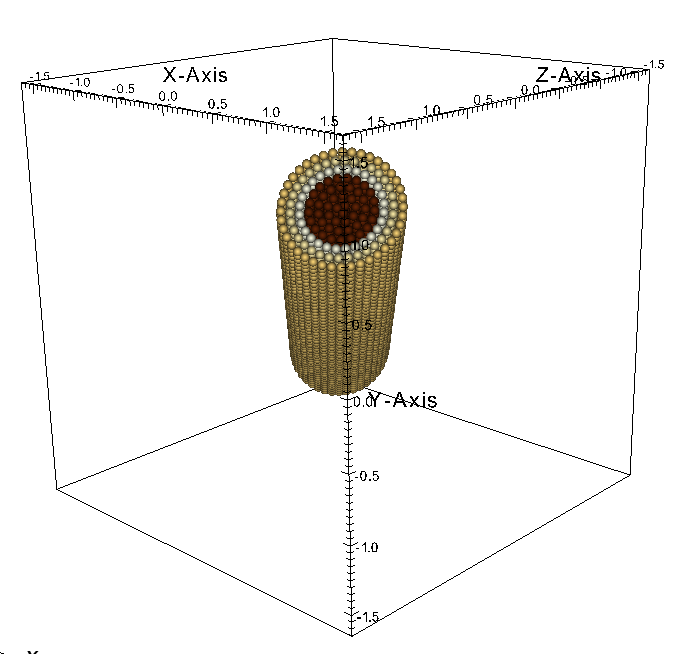
\includegraphics[width=0.9\columnwidth]{FIGS/geometry/geom_smooth_cyl_solid.png}
  \captionof{figure}{A \Textsfc{smoothcyl} geometry object. Particle volumes vary with radius.}
\end{minipage}

\begin{minipage}{0.6\textwidth}
  A hollow \Textsfc{smoothcyl} can be created by specifying an additional
  \Textsfc{thickness} parameter.  The thickness is required to be smaller than
  the radius.  The particle and grid resolution should be chosen such that the thickness
  contains at least two layers of particles.
  \begin{lstlisting}[language=XML]
    <smoothcyl label="cyl smooth">
      <bottom>[ -1.0, -1.0, -1.0]</bottom>
      <top>[ 1.0, 1.0, 1.0]</top>
      <radius> 0.5 </radius>
      <thickness> 0.2 </thickness>
    </smoothcyl>
  \end{lstlisting}
\end{minipage}
\begin{minipage}{0.4\textwidth}
  \centering
  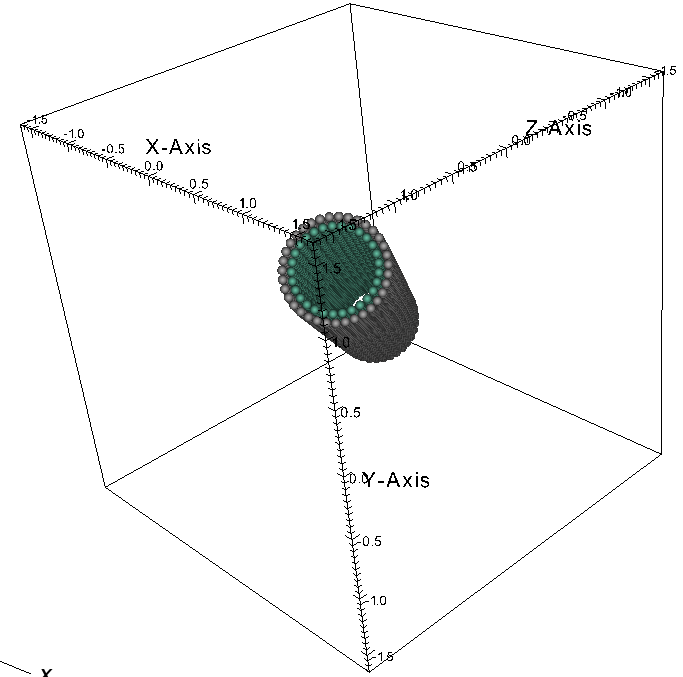
\includegraphics[width=0.9\columnwidth]{FIGS/geometry/geom_smooth_cyl_hollow.png}
  \captionof{figure}{A hollow \Textsfc{smoothcyl} geometry object.}
\end{minipage}

\begin{minipage}{0.6\textwidth}
  Endcaps can be added to the \Textsfc{smoothcyl} by specifying an additional
  \Textsfc{endcap thickness} parameter.  
  \begin{lstlisting}[language=XML]
    <smoothcyl label="cyl smooth">
      <bottom>[ -1.0, -1.0, -1.0]</bottom>
      <top>[ 1.0, 1.0, 1.0]</top>
      <radius> 0.5 </radius>
      <thickness> 0.2 </thickness>
      <endcap_thickness> 0.4 </endcap_thickness>
    </smoothcyl>
  \end{lstlisting}
\end{minipage}
\begin{minipage}{0.4\textwidth}
  \centering
  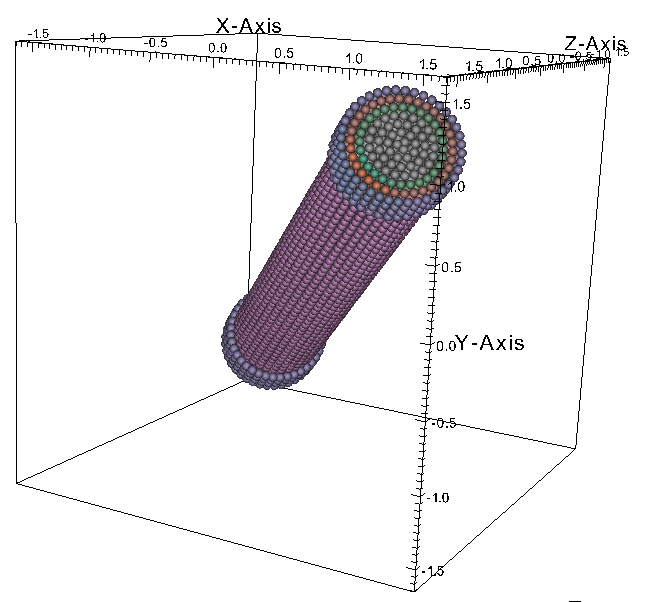
\includegraphics[width=0.9\columnwidth]{FIGS/geometry/geom_smooth_cyl_hollow_endcap.png}
  \captionof{figure}{A hollow \Textsfc{smoothcyl} with endcaps geometry object.}
\end{minipage}

\begin{minipage}{0.6\textwidth}
  Partial sectors of a \Textsfc{smoothcyl} can also be modeled by specifying \Textsfc{arc}
  information.  The start angle and arc angle default to 0 and 360 and have to be specified
  in degrees.
  The number of particles between \Textbfc{arc\_start} and \Textbfc{arc\_angle}
  is determined individually for each ring of particles by
  attempting to keep particle spacings approximately equal in the radial
  and angular directions, and thus particle volumes approximately
  constant.
  \begin{lstlisting}[language=XML]
    <smoothcyl label="cyl smooth">
      <bottom>[ -1.0, -1.0, -1.0]</bottom>
      <top>[ 1.0, 1.0, 1.0]</top>
      <radius> 0.5 </radius>
      <thickness> 0.2 </thickness>
      <endcap_thickness> 0.2 </endcap_thickness>
      <arc_start_angle_degree> 30 </arc_start_angle_degree>
      <arc_angle_degree> 90 </arc_angle_degree>
    </smoothcyl>
  \end{lstlisting}
\end{minipage}
\begin{minipage}{0.4\textwidth}
  \centering
  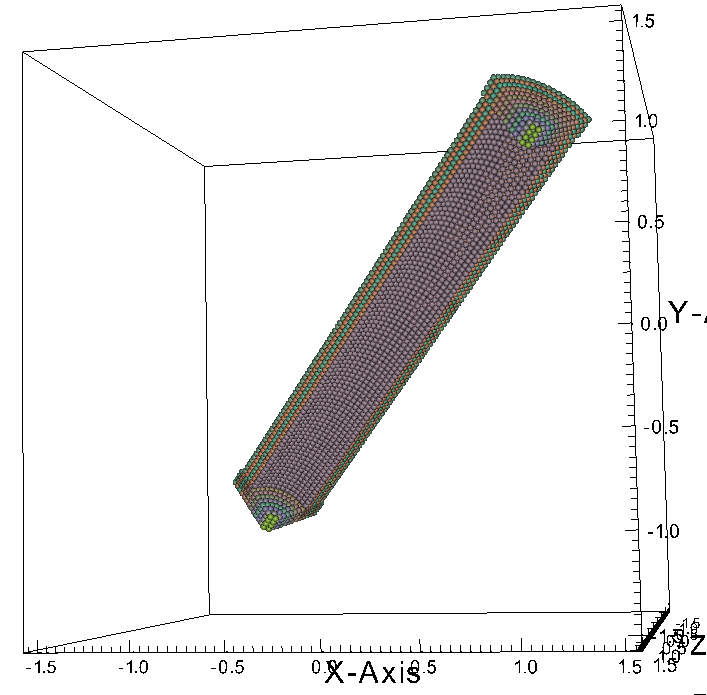
\includegraphics[width=0.9\columnwidth]{FIGS/geometry/geom_smooth_cyl_hollow_endcap_arc.png}
  \captionof{figure}{A partial hollow \Textsfc{smoothcyl} with endcaps.}
\end{minipage}

\begin{NoteBox}
Multiple \Textsfc{smoothcyl} geometries within a \Textbfc{\textless geom\_object\textgreater} 
tag are not
discretized using a body fit particle distribution as described here
(rather the default discretization scheme is used).  This will be
fixed eventually, at which point it may be possible to create more
general endcaps using unions of \Textsfc{smoothcyl}.
\end{NoteBox}

\subsection{Smooth sphere}
\begin{minipage}[t]{0.6\textwidth}
  \vspace{0pt}
  If quarter-symmetry simulations are not required, a smoother approximation
  to a sphere can be modeled using the \Textsfc{smooth\_sphere} tag. 
  The \Textsfc{center} tag specifies
  the center of the sphere, the \Textsfc{outer\_radius} tag is the outer radius, 
  \Textsfc{inner\_radius} the inner radius, and the 
  \Textsfc{num\_radial\_pts} tag indicates the number of points through the
  thickness.  Optionally, one can use the \Textsfc{algorithm} tag to determine
  which algorithm (\Textbfc{spiral} or \Textbfc{equal\_area}) 
  will be used to generate points and the \Textsfc{output\_file}
  tag to save the points and volume to a file that can be read in by the
  \Textsfc{file\_geometry} object creator.
  \begin{lstlisting}[language=XML]
    <smooth_sphere label="sphere_1">
      <center>[ 0.0, 0.0, 0.0]</center>
      <outer_radius> 1.0 </outer_radius>
      <inner_radius> 0.9 </inner_radius>
      <num_radial_pts> 5 </num_radial_pts>
      <algorithm> spiral </algorithm>
      <output_file> generated_sphere.pts </output_file>
    </smooth_sphere>
  \end{lstlisting}
\end{minipage}
\hspace{12pt}
\begin{minipage}[t]{0.35\textwidth}
  \vspace{0pt}
  \centering
  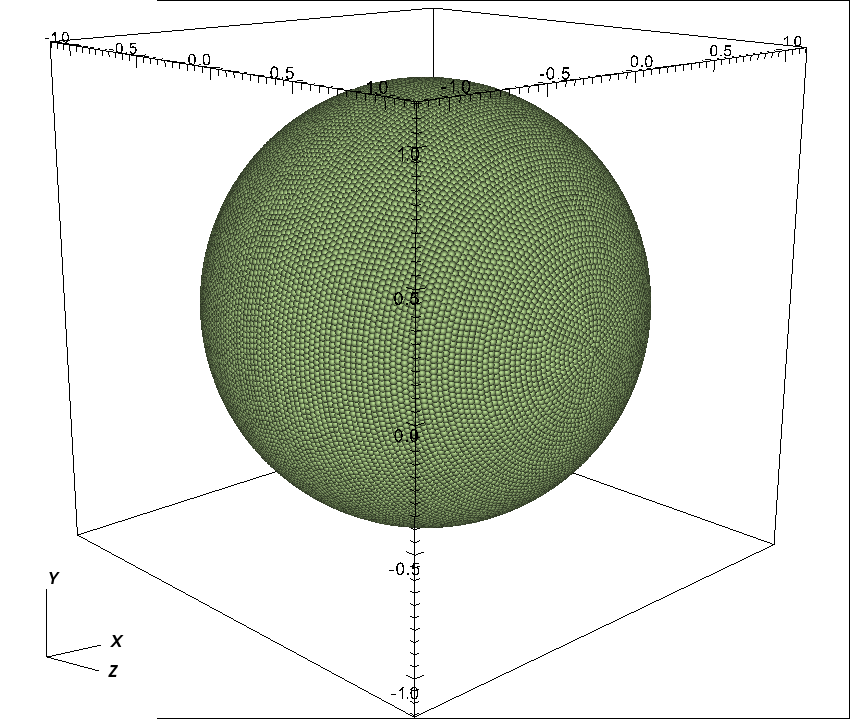
\includegraphics[width=0.9\columnwidth]{FIGS/geometry/geom_smooth_sphere.png}
  \captionof{figure}{A hollow \Textsfc{smooth\_sphere} geometry object generated
                     with the \Textsfc{spiral} algorithm.}
  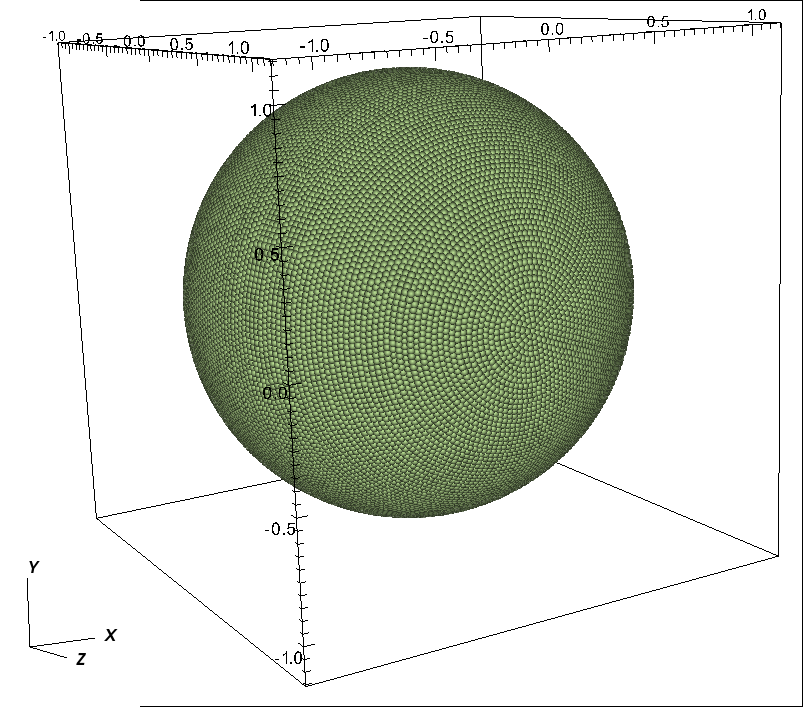
\includegraphics[width=0.9\columnwidth]{FIGS/geometry/geom_smooth_sphere_equal.png}
  \captionof{figure}{A hollow \Textsfc{smooth\_sphere} geometry object generated
                     with the \Textsfc{equal\_area} algorithm.}
\end{minipage}

\subsection{Spherical membrane}
\begin{minipage}{0.6\textwidth}
  The default discretization of a sphere leads to a rough approximation of the 
  surface of a sphere.  The \Textsfc{sphere\_membrane} geometry allows more
  control over the distribution of particles while retaining the possibility
  of modeling quarter symmetry spheres.  The \Textsfc{origin} tag specifies
  the center of the sphere, the \Textsfc{radius} tag is the outer radius, 
  the \Textsfc{thickness} the thickness of the sphere wall, the 
  \Textsfc{num\_lat} label the number of points along the latitude and
  \Textsfc{num\_long} label indicates the number of points along the longitude.
  \begin{lstlisting}[language=XML]
    <sphere_membrane label="membrane">
      <origin>[ 0.0, 0.0, 0.0]</origin>
      <radius> 1.0 </radius>
      <thickness> 0.1 </thickness>
      <num_lat> 10 </num_lat>
      <num_long> 10 </num_long>
    </sphere_membrane>
  \end{lstlisting}
\end{minipage}
\hspace{12pt}
\begin{minipage}{0.35\textwidth}
  \centering
  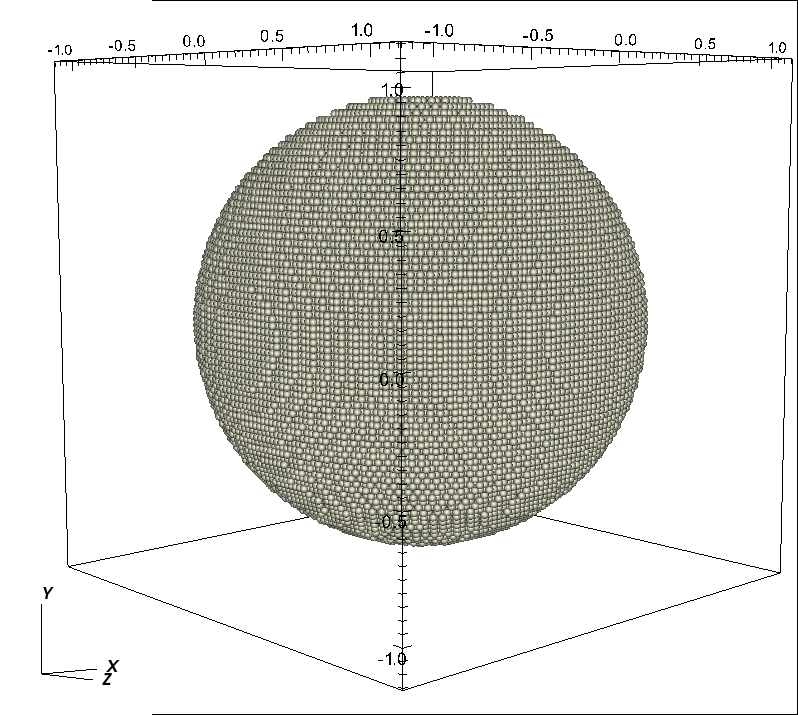
\includegraphics[width=0.7\columnwidth]{FIGS/geometry/geom_sph_mem.png}
  \captionof{figure}{A hollow \Textsfc{sphere\_membrane} geometry object.}
\end{minipage}

\subsection{Corrugated edge}
\begin{minipage}[t]{0.6\textwidth}
  \vspace{0pt}
  The \Textsfc{corrugated} tag creates a plate with one corrugated edge.  The particle spacing
  is determined from the grid size and the number of particles per grid cell.
  The input requires the minimum and maximum limits of the plate \Textsfc{xymin} and
  \Textsfc{xymax}, the \Textsfc{thickness}, the plate \Textsfc{normal}, the 
  \Textsfc{corr\_edge} edge that is to be corrugated (values of \Textbfc{x+}, \Textbfc{y+},
  \Textbfc{x-}, and \Textbfc{y-} are allowed), the type of \Textsfc{curve} (\Textbfc{sin}
  or \Textbfc{cos}), the \Textsfc{wavelength} and the \Textsfc{amplitude} of the 
  corrugation.  A sample input can be:
  \begin{lstlisting}[language=XML]
    <corrugated> 
      <xymin>      [0.0,0.0,0.0]    </xymin> 
      <xymax>      [20.0,20.0,0.0]  </xymax> 
      <thickness>  1.0              </thickness>
      <normal>     [0.0,0.0,1.0]    </normal>
      <corr_edge>  x+               </corr_edge>
      <curve>      sin              </curve>
      <wavelength> 2.0              </wavelength>
      <amplitude>  2.0              </amplitude>
    </corrugated>
  \end{lstlisting}
\end{minipage}
\hspace{12pt}
\begin{minipage}[t]{0.35\textwidth}
  \vspace{0pt}
  \centering
  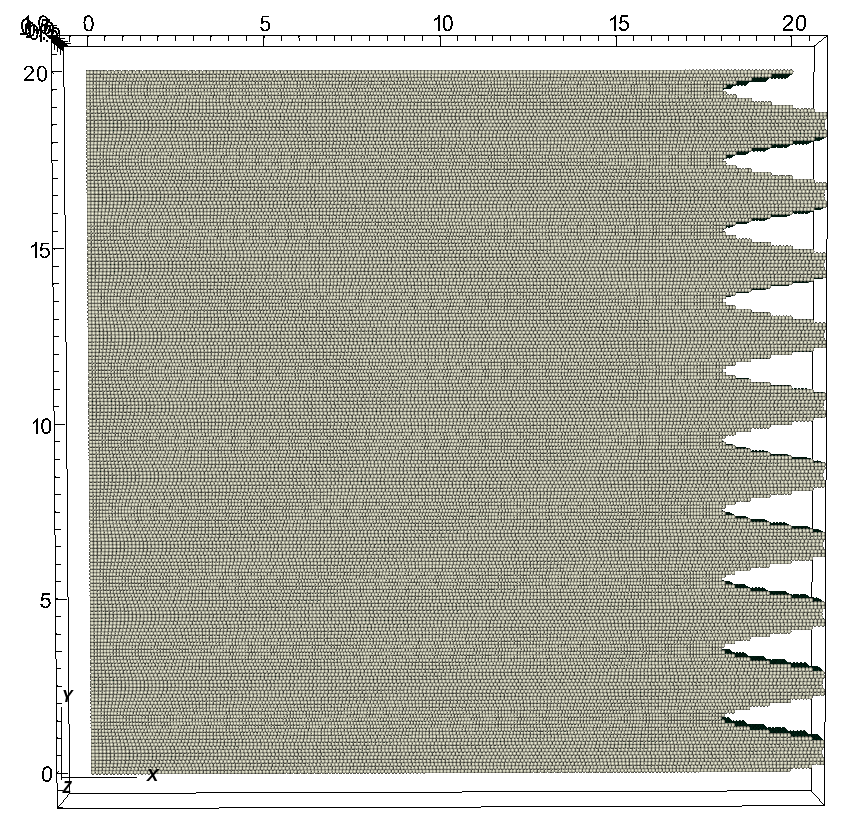
\includegraphics[width=0.7\columnwidth]{FIGS/geometry/geom_corrug.png}
  \captionof{figure}{A \Textsfc{corrugated} edge geometry object.}
\end{minipage}

\subsection{Specifying particle locations directly}
\begin{minipage}[t]{0.6\textwidth}
  \vspace{0pt}
  In addition to the above, it is also possible in MPM simulations to describe
  geometry by providing a file containing a series of particle locations.  These
  can be in either ASCII or binary format.  In addition, it is also possible to
  provide initial data for certain variables on the particles, including
  volume, temperature, external force, fiber direction (used in material models
  with transverse isotropy) and velocity.  The following is an example in which
  external force and fiber direction are specified:
  \begin{lstlisting}[language=XML]
    <file>
      <name>LVcoarse.pts</name>
      <var>p.externalforce</var>
      <var>p.fiberdir</var>
    </file>
  \end{lstlisting}
\end{minipage}
\hspace{12pt}
\begin{minipage}[t]{0.35\textwidth}
  \vspace{0pt}
  \centering
  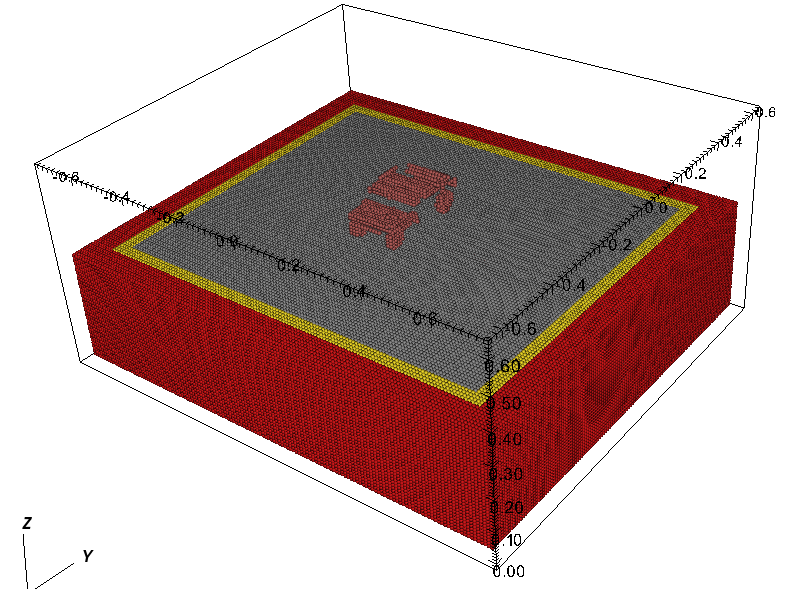
\includegraphics[width=0.9\columnwidth]{FIGS/geometry/geom_file_input.png}
  \captionof{figure}{A \Textsfc{file} based geometry object.}
\end{minipage}

  The text file \Textsfc{LVcoarse.pts} looks like:
  \begin{lstlisting}[backgroundcolor=\color{background}]
  0.0385 0.0335 0.0015 0 0 0 0.248865 -0.0593421 -0.966718
  0.0395 0.0335 0.0015 0 0 0 0.254892 -0.0220365 -0.966718
  0.0405 0.0335 0.0015 0 0 0 0.267002 0.0197728 -0.963493
  0.0415 0.0335 0.0015 0 0 0 0.261177 0.0588869 -0.963493
  ...
  \end{lstlisting}
  Because these files can be arbitrarily large, an additional preprocessing step
  must be taken before issuing the \Textsfc{vaango} command.
  \Textsfc{particleFileSplitter} is a utility that splits the
  data in the \Textsfc{.pts} file into a series of files
  (\Textsfc{file.pts.0, file.pts.1,}, etc), one for each
  patch.  By doing this, each processor needs only read in the data for the
  patches that it contains, rather than each processor reading in the entire file,
  which can be hard on the file system.  Note, that this step is required,
  even if only using a single patch, and must be reissued any time the patch
  configuration is changed.  Usage of this utility, which is compiled
  into the \Textsfc{StandAlone/particleFileSplitter} executable, is:
  \begin{lstlisting}[backgroundcolor=\color{background}]
     particleFileSplitter input.ups
  \end{lstlisting}

  An associated utility that can be used to extract particle position and
  volume information from a \Textsfc{UDA} file is
  \Textsfc{StandAlone/createFileGeomPieceFromUda}. An example of its usage
  is
  \begin{lstlisting}[backgroundcolor=\color{background}]
  createFileGeomPieceFromUda file_geom_pfs_hummer_inp.uda.000 file_geom_pfs_hummer.dat
  \end{lstlisting}
  This utility extracts the material points and their volumes into files with
  a \Textbfc{mat} suffix.  For example, for an input file containing 6 materials,
  the extracted files are named:
  \begin{lstlisting}[backgroundcolor=\color{background}]
    file_geom_pfs_hummer.dat.mat0
    file_geom_pfs_hummer.dat.mat1
    file_geom_pfs_hummer.dat.mat2
    file_geom_pfs_hummer.dat.mat3
    file_geom_pfs_hummer.dat.mat4
    file_geom_pfs_hummer.dat.mat5
  \end{lstlisting}
  We can now create another input file \Textsfc{file\_geom.ups}
  containing the \Textsfc{file} geometry objects and two patches:
  \begin{lstlisting}[language=XML]
    <geom_object>
      <file label = "container">
        <name> file_geom_pfs_hummer.dat.mat0 </name>
        <var> p.volume </var>
      </file>
      <res>[2,2,2]</res>
      <velocity>[0.0,0.0,-10]</velocity>
      <temperature>300</temperature>
    </geom_object>
    <geom_object>
      <file label = "base">
        <name> file_geom_pfs_hummer.dat.mat1 </name>
        <var> p.volume </var>
      </file>
      <res>[2,2,2]</res>
      <velocity>[0.0,0.0,-10]</velocity>
      <temperature>300</temperature>
    </geom_object>
    ...
  \end{lstlisting}
  To activate these objects we run \Textsfc{particleFileSplitter}:
  \begin{lstlisting}[backgroundcolor=\color{background}]
     particleFileSplitter file_geom.ups
  \end{lstlisting}
  to get the split files
  \begin{lstlisting}[backgroundcolor=\color{background}]
    file_geom_pfs_hummer.dat.mat0.0
    file_geom_pfs_hummer.dat.mat0.1
    file_geom_pfs_hummer.dat.mat1.0
    file_geom_pfs_hummer.dat.mat1.1
    ....
  \end{lstlisting}
  After this step we can run the usual \Vaango simulation with
  \begin{lstlisting}[backgroundcolor=\color{background}]
    mpirun -np 2 vaango file_geom.ups
  \end{lstlisting}
  

\subsection{Using image data to create particles}
\begin{minipage}[t]{0.6\textwidth}
  \vspace{0pt}
  One final option is available for initializing particle positions in \MPM
  simulations, and that is through the use of three-dimensional image data,
  such as might be collected via microCT scans or confocal microscopy.  The image data are 
  provided as 2-byte (16-bit/short) raw files, and usage in the input file is given as:
  \begin{lstlisting}[language=XML]
    <geom_object>
      <image>
        <name> Almond_Kiss_2003112600.raw </name>
        <res> [425, 420, 260] </res>
        <threshold> [11, 200] </threshold>
      </image>
      <file label = "container">
        <name> Almond_Kiss_2003112600.pts </name>
        <format> bin </format>
      </file>
      <res>[1,1,1]</res>
      <velocity>[0.0,0.0,-10]</velocity>
      <temperature>300</temperature>
    </geom_object>
  \end{lstlisting}
\end{minipage}
\hspace{12pt}
\begin{minipage}[t]{0.35\textwidth}
  \vspace{0pt}
  \centering
  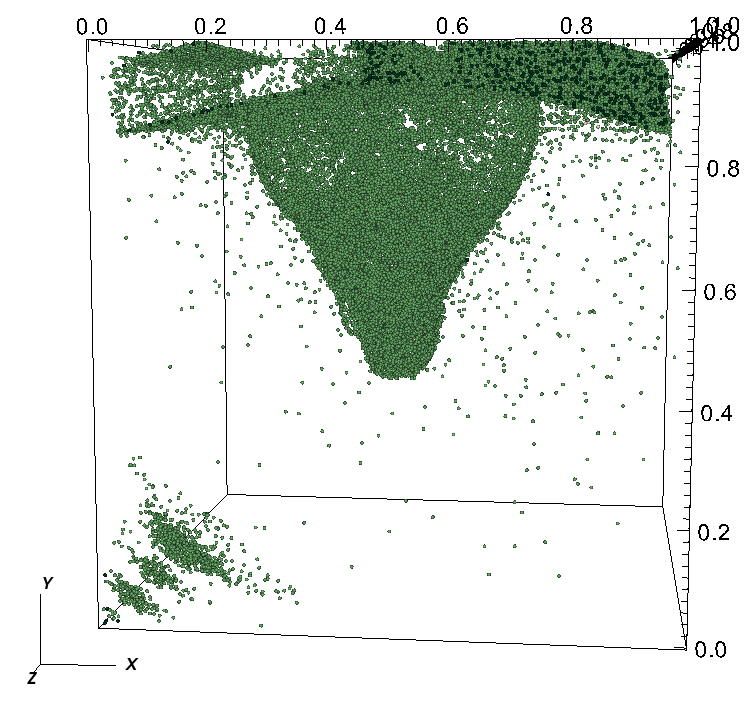
\includegraphics[width=0.9\columnwidth]{FIGS/geometry/geom_image.png}
  \captionof{figure}{An \Textsfc{image} and \Textsfc{file} based geometry object.}
\end{minipage}

  Note that the \Textsfc{geom\_object} resolution is typically given as $[1,1,1]$. 
  The \Textsfc{\textless image\textgreater} section gives the name of the 3D image file, 
  the resolution of the image in pixels in the various coordinate directions, and 
  a threshold range.  Particles will be generated at voxels within the specified range.  
  The \Textsfc{\textless file\textgreater} section is the same as that described earlier.  

  The \Textsfc{level} section in the input file also requires the same resolution for
  consistency.  For example, 
  \begin{lstlisting}[language=XML]
    <Level>
      <Box label = "1">
        <lower>[0, 0, 0]</lower>
        <upper>[1, 1, 1]</upper>
        <resolution>[425, 420, 260]</resolution>
        <patches>[1,1,1]</patches>
        <extraCells>[1,1,1]</extraCells>
      </Box>
    </Level>
  \end{lstlisting}

  A different preprocessing utility is needed when using image data (for the same reasons 
  described previously).  Usage is as follows:
  \begin{lstlisting}[backgroundcolor=\color{background}]
     particleImageFileSplitter -b input.ups
  \end{lstlisting}
  The \Textbfc{-b} flag indicates that binary \Textsfc{spheres.pts.\#} files will be created, which
  saves considerable disk space when performing large simulations.

  \begin{NoteBox}
   A convenient tool for creating \Textsfc{raw} image files is the Slicer3D software
   which can be downloaded from \url{https://www.slicer.org/}.  If the microCT image
   is loaded into Slider3D, it can be converted into NRRD format with separate files
   for the header (extension \Textbfc{nrhd}).  If the compression option is turned off
   while saving as \Textbfc{nrhd}, a raw file containing 16-bit pixel values is created.
   This file can be used as input to \Vaango.
  \end{NoteBox}

